
\documentclass[12pt, openany]{book}
\usepackage{graphicx}
\usepackage{amsmath}
\usepackage{amssymb}
\usepackage{amsthm}
\usepackage{enumitem}
\usepackage{titlesec}
\usepackage{fancyhdr}
\usepackage{geometry}
\usepackage{xcolor}
\usepackage{color}
\usepackage{listings}
\usepackage{float}
\usepackage{hyperref}
\usepackage{booktabs}

% Page layout
\geometry{a4paper, margin=1in}
\pagestyle{fancy}
\fancyhf{}
\fancyhead[L]{\leftmark}
\fancyhead[R]{\thepage}
\renewcommand{\headrulewidth}{0.4pt}

% Chapter formatting
\titleformat{\chapter}[display]
{\normalfont\huge\bfseries}
{\chaptertitlename\ \thechapter}{20pt}{\Huge}

% Custom colors
\definecolor{codegray}{rgb}{0.5,0.5,0.5}
\definecolor{codepurple}{rgb}{0.58,0,0.82}
\definecolor{backcolour}{rgb}{0.95,0.95,0.92}  % Light gray background

% Listings configuration
\lstdefinestyle{mystyle}{
    backgroundcolor=\color{backcolour},
    commentstyle=\color{codegray},
    keywordstyle=\color{codepurple},
    numberstyle=\tiny\color{codegray},
    stringstyle=\color{codepurple},
    basicstyle=\ttfamily\footnotesize\color{black},  % Explicitly set text color
    breakatwhitespace=false,
    breaklines=true,
    captionpos=b,
    keepspaces=true,
    numbers=left,
    numbersep=5pt,
    showspaces=false,
    showstringspaces=false,
    showtabs=false,
    tabsize=2
}
\lstset{style=mystyle}

% Remove footers with professor name
\fancyfoot{}
\renewcommand{\rmdefault}{qpl}

\begin{document}

\setcounter{page}{45}
\setcounter{chapter}{4}
\chapter{Big Data Frameworks - RDD}

\section{CSE6001}

BIG DATA FRAMEWORKS


Module -


RDD


Prof. Lokeshkumar R


\section{Spark Memory Management}
\begin{itemize}[leftmargin=*]\item Memory utilization is essential in Spark

(Caching)

\item Spark process is a JVM process\end{itemize}

\begin{figure}[H]
\centering
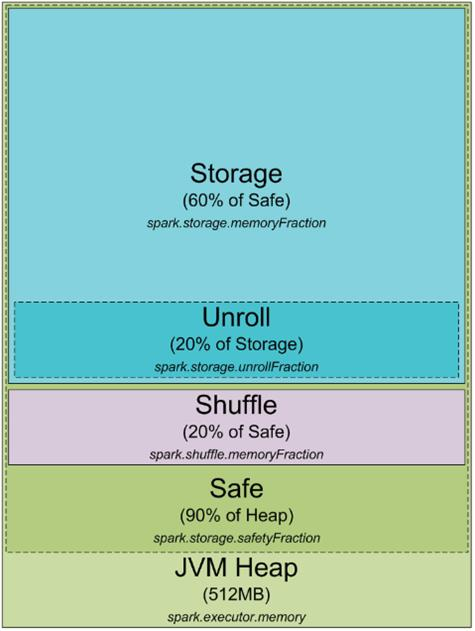
\includegraphics[width=0.8\textwidth]{pdf_images_output/img_p2_xref19.jpeg}
\caption{Diagram related to: Spark Memory Management}
\end{figure}

\section{Spark Programming Model}
\begin{itemize}[leftmargin=*]\item High-Level coding to build a workflow  (Scala)
\item Code compiles to distributed parallel operations
\item Two Abstraction Units
\item RDDs: Resilient Distributed Datasets
\item Parallel Operations\end{itemize}

\section{RDD: Concept}
\begin{itemize}[leftmargin=*]\item Collection of objects (records) that act as one unit
\item Stored in main memory or disk
\item Parallel operations built on top of them
\item Have fault tolerance without replication (lineage)\end{itemize}

\begin{itemize}[leftmargin=*]\item RDD is read-only
\item Distributed either in main memory or disk (automatically

decided)
\end{itemize}

\begin{figure}[H]
\centering
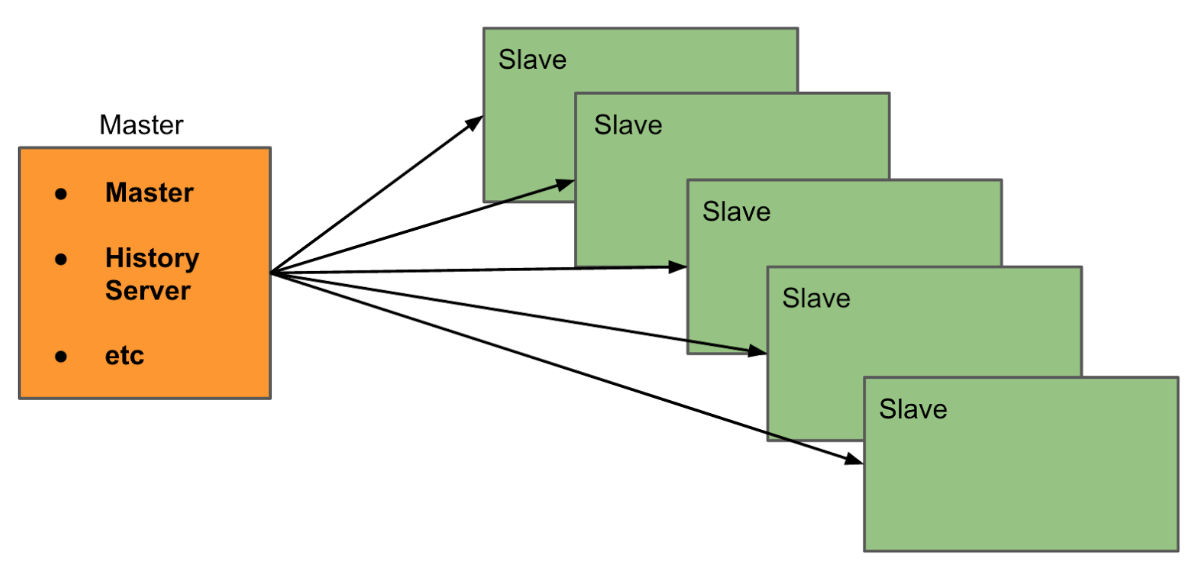
\includegraphics[width=0.8\textwidth]{pdf_images_output/img_p5_xref33.png}
\caption{Diagram related to: RDD: Concept}
\end{figure}

\begin{figure}[H]
\centering

\includegraphics[width=0.8\textwidth]{pdf_images_output/img_p5_xref34.jpeg}
\caption{Diagram related to: RDD: Concept}
\end{figure}

\section{RDD vs. Traditional Shared Memory}


\begin{figure}[H]
\centering
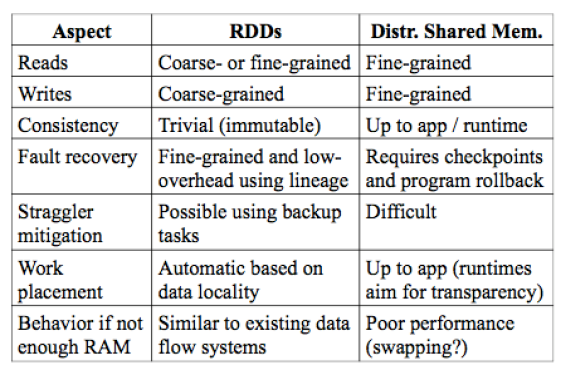
\includegraphics[width=0.8\textwidth]{pdf_images_output/img_p6_xref37.png}
\caption{Diagram related to: RDD vs. Traditional Shared Memory}
\end{figure}

\section{Why do we need RDD in Spark?}
\begin{itemize}[leftmargin=*]\item The key motivations behind the concept of RDD are-

Iterative algorithms.


Interactive data mining tools


DSM (Distributed Shared Memory) is a very general abstraction,


but this generality makes it harder to implement in an efficient and


fault tolerant manner on commodity clusters. Here the need of


RDD comes into the picture.


In distributed computing system data is stored in intermediate


stable distributed store such as HDFS or Amazon S3. This makes the


computation of job slower since it involves many IO operations,


replications, and serializations in the process.
\end{itemize}

\section{Why do we need RDD in Spark?(1)}
\begin{itemize}[leftmargin=*]\item The main challenge in designing RDD is defining a program interface

that provides fault tolerance efficiently.

\item To achieve fault tolerance efficiently, RDDs provide a restricted form

of shared memory, based on coarse-grained transformation rather


than fine-grained updates to shared state.

\item Spark exposes RDD through language integrated API.
\item In integrated API each data set is represented as an object and

transformation is involved using the method of these objects.
\end{itemize}

\section{Features of Spark RDD}
\begin{itemize}[leftmargin=*]\item In-memory Computation
\item Lazy Evaluations
\item Fault Tolerance
\item Immutability
\item Partitioning
\item Persistence
\item Location-Stickiness\end{itemize}

\section{In-memory Computation}
\begin{itemize}[leftmargin=*]\item Spark RDDs have a provision of in-memory computation. It stores

intermediate results in distributed memory(RAM) instead of stable


storage(disk).


Lazy Evaluations


All transformations in Apache Spark are lazy, in that they do not compute


their results right away. Instead, they just remember the transformations


applied to some base data set.
\end{itemize}

\section{Fault Tolerance}
\begin{itemize}[leftmargin=*]\item Spark RDDs are fault tolerant as they track data lineage information to

rebuild lost data automatically on failure. They rebuild lost data on


failure using lineage, each RDD remembers how it was created from


other datasets (by transformations like a map, join or groupBy) to


recreate itself.


Immutability

\item Data is safe to share across processes. It can also be created or

retrieved anytime which makes caching, sharing \& replication easy.


Thus, it is a way to reach consistency in computations.
\end{itemize}

\section{Partitioning}
\begin{itemize}[leftmargin=*]\item Partitioning is the fundamental unit of parallelism in Spark RDD. Each

partition is one logical division of data which is mutable. One can


create


a


partition


through


some


transformations


on


existing


partitions.


Persistence

\item Users can state which RDDs they will reuse and choose a storage

strategy for them (e.g., in-memory storage or on Disk).
\end{itemize}

\section{Coarse-grained Operations}
\begin{itemize}[leftmargin=*]\item It applies to all elements in datasets through maps or filter or group

by operation.


Location-Stickiness

\item RDDs are capable of defining placement preference to compute

partitions. Placement preference refers to information about the


location of RDD. The DAGScheduler places the partitions in such a


way that task is close to data as much as possible. Thus, speed up


computation
\end{itemize}

\section{Spark RDD Operations}
\begin{itemize}[leftmargin=*]\item Transformation
\item Spark RDD Transformations are functions that take an RDD as the input and

produce one or many RDDs as the output.

\item They do not change the input RDD (since RDDs are immutable and hence one

cannot change it), but always produce one or more new RDDs by applying the


computations they represent e.g. Map(), filter(), reduceByKey() etc.

\item Narrow Transformations
\item Wide Transformations
\item Actions\end{itemize}

\section{Narrow Transformations}
\begin{itemize}[leftmargin=*]\item It is the result of map, filter and such that the data is from a single

partition only, i.e. it is self-sufficient. An output RDD has partitions


with records that originate from a single partition in the parent RDD.


Only a limited subset of partitions used to calculate the result.
\end{itemize}

\begin{figure}[H]
\centering
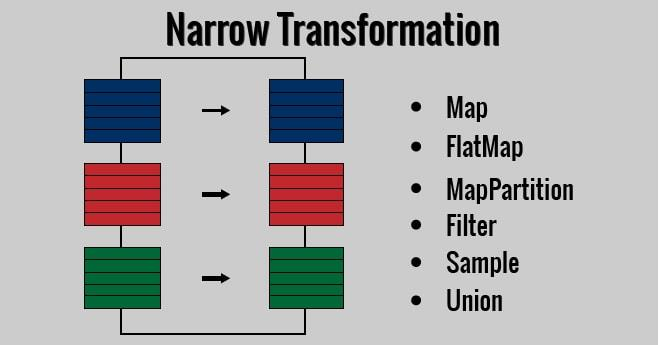
\includegraphics[width=0.8\textwidth]{pdf_images_output/img_p15_xref65.jpeg}
\caption{Diagram related to: Narrow Transformations}
\end{figure}

\section{Wide Transformations}
\begin{itemize}[leftmargin=*]\item It is the result of groupByKey() and reduceByKey() like functions. The data

required to compute the records in a single partition may live in many


partitions of the parent RDD. Wide transformations are also known


as shuffle transformations because they may or may not depend on a


shuffle.
\end{itemize}

\begin{figure}[H]
\centering
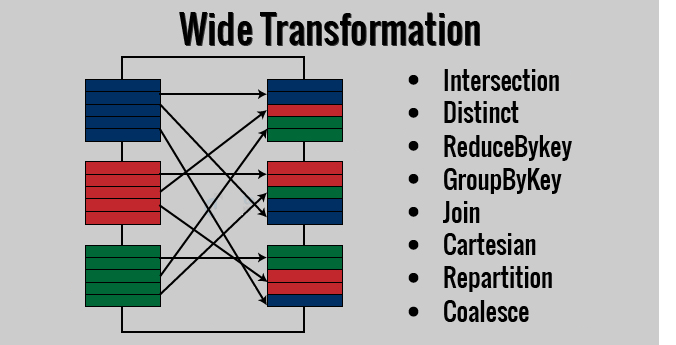
\includegraphics[width=0.8\textwidth]{pdf_images_output/img_p16_xref68.png}
\caption{Diagram related to: Wide Transformations}
\end{figure}

\section{Actions}
\begin{itemize}[leftmargin=*]\item An Action in Spark returns final result of RDD computations.
\item It triggers execution using lineage graph to load the data into original

RDD, carry out all intermediate transformations and return final


results to Driver program or write it out to file system.

\item Lineage graph is dependency graph of all parallel RDDs of RDD.
\item Actions are RDD operations that produce non-RDD values. They

materialize a value in a Spark program.

\item An Action is one of the ways to send result from executors to

the driver. First(), take(), reduce(), collect(), the count() is some of the


Actions in spark.
\end{itemize}

\end{document}
